\section{Evaluation} \label{section:evaluation}
We conducted a user study to compare \tool to a \baseline tool. \baseline only contains the features present in current property booking tools (e.g. Airbnb \cite{airbnb} or Booking.com \cite{booking}) and collaborative search tools (e.g. SearchTogether \cite{searchtogether} or ResultsSpace \cite{resultsspace}). It contains a search page along with the \collabQueryPanel, a chat, and a bookmarks page that shows a list of bookmarked properties. The bookmarks page is similar to Airbnb's wishlists or the summary section of SearchTogether~\cite{searchtogether}.  \baseline has a similar UI aesthetic to \tool.  

The goal of our study is to  (i) assess if users of \tool can reach more satisfying agreements when compared to \baseline, (ii) determine if there are differences across both tools in how and when users conduct the different tasks (Section \ref{ssection:task}) associated with group booking, (iii) qualitatively evaluate the utility of \tool's novel features in the context of the challenges (Section \ref{ssection:challenges}) we identified from our formative conversations and study.

\subsection{Methodology} \label{ssection:methodology}
Twenty-one participants were recruited to use \tool, and twenty-one were recruited to use \baseline. User study participants were recruited from a university's academic and residential (student, staff, faculty and affiliate) campuses and mailing lists. The lists' subscribers included former and current university employees, alumni and students. Participants recruited  were between the ages of 18 and 37, 50.0\% identified as female and 50.0\% as male.  85.7\% have a high school diploma and 14.3\% have a college degree or higher. 69.0\% reported having experience collaborating with people over the web. 

Participants took part in a zoom session where they received a tutorial on \tool or \baseline. Participants were encouraged to ask clarifying questions at all times during the tutorial session to ensure proficiency with the tool. In addition, participants had access to video tutorials prepared by the researchers. Any emailed questions were answered at the researchers' earliest convenience throughout the duration of the multiple-day study. 

Participants were asked to complete a pre-experiment questionnaire where they signed a consent form and reported simple biographical information (i.e. age, gender, and education) and their experience with search and digital collaboration. 

To ensure the participants are committed to the task at hand, a commitment akin to that of an enthusiastic tenant-to-be rigorously searching as they are to make a substantial time and financial investment, participants were tasked with being the personal-shopper of an avatar that has specific requirements for their home. The avatars' descriptions are attached in Appendix \ref{appendix:avatars}. The participants were then placed in a random anonymous group of 3 participants, each representing an avatar. The participant in the group that best represented their avatar's requirements in the final selected property received a monetary bonus. We acknowledge that the participants in this study do not elicit the same sense of personal investment as the avatars they represent would in real life. The avatar user study provides a controlled environment that allowed us to accommodate a variety of testing conditions particular to \tool. More specifically, it allowed us to study the effects of conflicting preferences in group dynamics and decision-making (e.g. smoking vs not-smoking or conflicting budgetary constraints as seen in Appendix \ref{appendix:avatars}). It gave us flexibility in recruiting participants and pairing them in groups with ease and at scale. Finally, the monetary reward gave participants a motivating drive to push for their avatar's interests within the group. 

Participants were told to look for a property in New York City for a week-long vacation using \tool. \tool's database was populated with properties from New York City to resemble as close as possible a real-life scenario. 

Participants participated in the study asynchronously and remotely for up to 5 days. Participants were asked to log in periodically to the tool and search with their team members. No form of micro-management or timing requirements were imposed. The anonymity of the participants ensured that the tool itself was the only communication medium amongst the team members. 

Users using \tool were asked to come to an agreement by all of them signing a contract. Users using \baseline were asked to send a screenshot of the final agreed upon property via email to the researchers as the tool did not possess an embedded agreement system. 

After concluding the study, participants were asked to complete a post-experiment questionnaire where they rated the tools they used and the features contained wherein. After the participants completed the questionnaire, their participation payment and any earned bonuses were processed. 

\subsection{Results} \label{ssection:results}
We begin by stating that our results must be taken with a grain of salt: Our positive results are simply promising indications that \tool's design does support collaborative property search and agreement; Our surfaced patterns and observations are exciting, but merit future confirmatory research. Our study size is relatively small though not unusual for HCI studies of this nature (e.g. 14 participants for SearchTogether \cite{searchtogether} and 14 participants for ResultsSpace  \cite{TeamSearch}). Please refer to Table \ref{tab:lit-comparison} for a more comprehensive comparison between \tool and previous work. 

Small study size is due to the challenges involved in recruiting and managing participants for a collaborative, effort- and time-intensive, multi-day study. While we provide statistics in our presentation, we use those as brief summaries of our qualitative observations rather than as representative statistics of the population that may use \tool. 


\subsubsection{Can users of \tool reach more satisfying agreements when compared to \baseline?}
\begin{itemize}
    \item All seven groups with three participants each using \tool  signed a contract.
    \item Six of the seven groups of three using \baseline were able to agree on a property within the study.
\end{itemize}

Based on a 5-point Likert scale question that asked users to rate their overall degree of satisfaction with the property chosen by the group in the post-study questionnaire,
\begin{itemize}
    \item The average rating across users using \tool was 4.52 ($\sigma = 0.67$).
    \item The average rating across users using \baseline was 3.88 ($\sigma = 1.02$).
\end{itemize}

The reported success of \tool in reaching a satisfying agreement is also corroborated by whether or not the users were able to satisfy the requirements specified by their Avatar. As seen in Appendix \ref{appendix:avatars}, each avatar had 4 requirements for their dream home. In \tool, the average number of satisfied requirements was 2.52 ($\sigma = 0.46$) and in \baseline it was 2 ($\sigma = 3.06$). This number is quite high considering that the avatars had conflicting smoking preferences, meaning it was impossible for all avatars to achieve all 4 of their requirements.

\subsubsection{Are there differences in how and when users conduct tasks across the tools?}

To understand differences in user behaviour across both tools, we instrumented them to track as many activities as possible on the user interface. These activities included log-ins, clicking on any button or link or sending a chat message. Certain activities could not be tracked e.g how long each user dwelled on search results or scrolled through them, or if/when they logged-out. This tracking is facilitated by \tool's system architecture described in Figure \ref{fig:crest-architecture}. Not only do we save every single user action that occurs within \tool in our database as a byproduct of implementing a full-stack tool, but we also implement a dedicated logging service that tracks all major events (i.e. "User 1 added preference refrigerator in Team 2") in a table in our database.

We then grouped each of these tracked activities into the three main actions involved in group booking: search, discuss and agree. \textit{Search} included activities like adding, modifying, liking or disliking a user preference, clicking on a property for more details, bookmarking it, etc. Two of the authors conducted a natural language analysis of the messages to classify them into the two remaining categories: \textit{Discuss} and \textit{Agree}. Both authors used a simple heurestic to aid this labeling: if a message mentioned a specific property, it was most likely seeking agreement on it and was often labeled 'agree', other messages were often labeled 'discuss.'

\begin{figure}
    \centering
    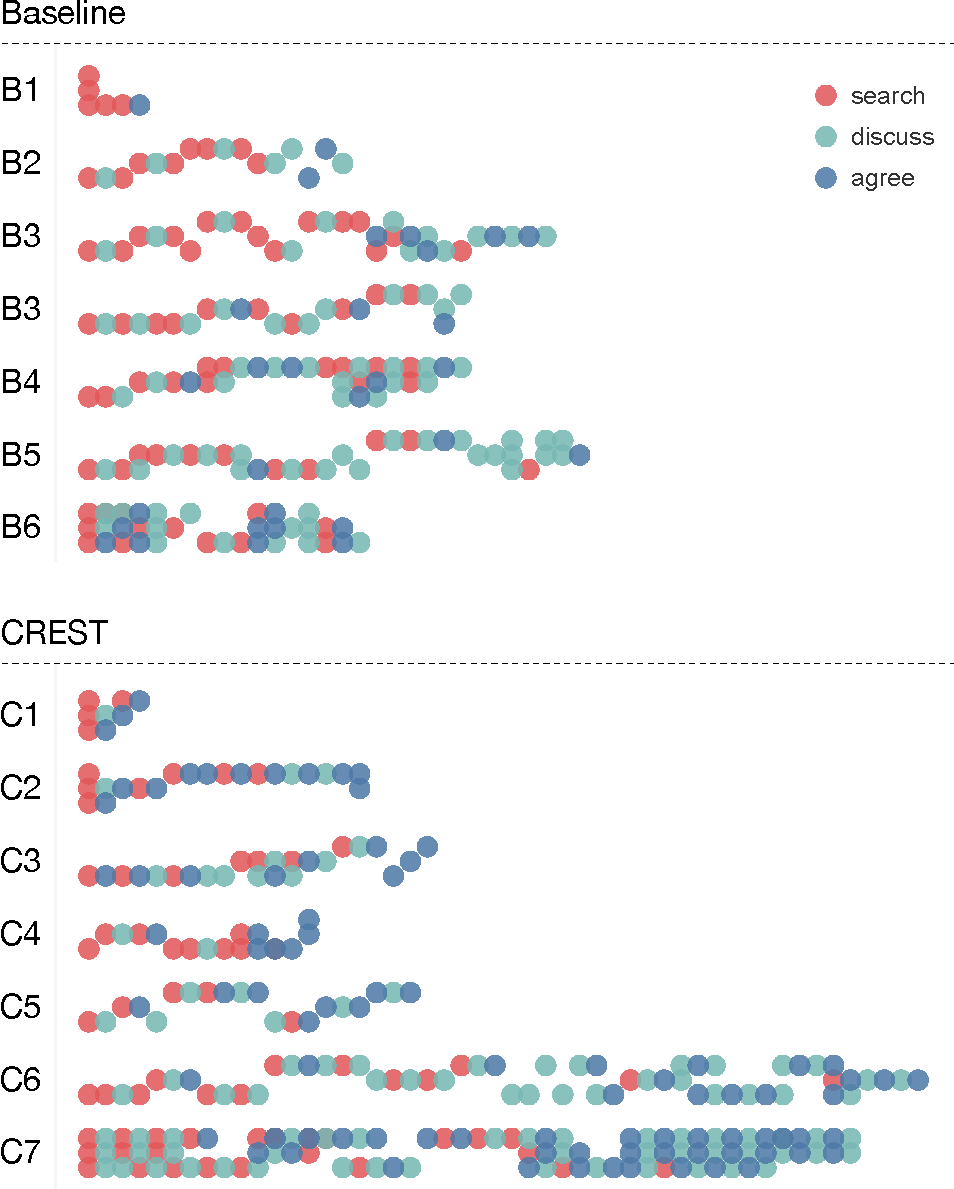
\includegraphics[width=1\linewidth]{images/logical-timelines.pdf}
    \caption{An overview of the sequence of events that occurred in each group across its three users. Users are ordered vertically. Events are logically ordered along the horizontal order axis. A single event captures one or more consecutive actions of a task type (search, discuss or agree) that occured within a user's session. In situations where users were active during the same time span, their events might have the same logical order. We opt for logical order instead of physical timestamps due to the asynchronous, multi-day nature of the study: users were disconnected for large time periods with infrequent bursts of activity. B6 is the only group that failed to agree on a property to book.}
    \label{fig:timelines}
\end{figure}

Figure \ref{fig:timelines} illustrates how the collaborative booking progessed within each of 14 teams. We note the asynchronous nature of the study with users often being active at different times. 

We provide the figure for reference noting that it is difficult to infer general patterns from fine-granularity sequences. However, we can observe that most sequences begin with users alternating between search and discussion tasks and then conclude with users alternating between discussion and agreement tasks. We find users engaging in more agreement activities with \tool than in the \baseline. B6 is the only group that failed to book a specific property at the end of the study.

We observe that groups using \tool engage in agreement activities earlier than in \baseline. To better visualize this phenonema, we normalized all event sequences on a scale of 0-100 and then for each group plotted when the first agreement event occurred as follows:\\
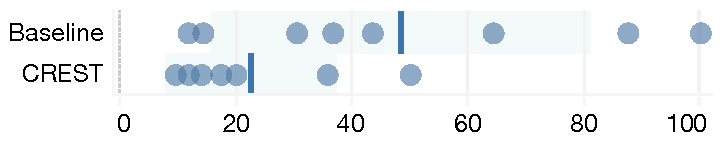
\includegraphics[height=42px]{images/Norm_Agreement_Start.pdf}\\[0.1cm]
This possibly alludes to the efficacy of \tool's goal-centered design at driving group members towards collaborative agreement. 

Similary, we plotted the last search event for each group. \\[0.1cm]
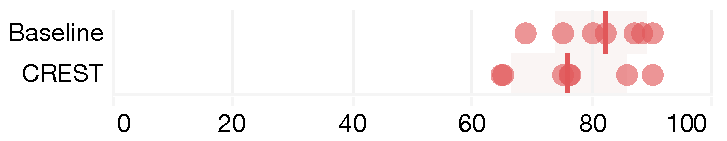
\includegraphics[height=42px]{images/SearchEnd.pdf}\\
We find some indication of a more extended search in the \baseline hinting at the shifting goal posts challenge. We find that engaging in agreement activities earlier in \tool does not limit exploration. On average, \baseline teams created 6.71 ($\sigma = 2.63$) bookmarks and \tool teams created 6.43 ($\sigma = 3.05$) contracts. Compared to proposing contracts, bookmarking a property is a simpler action to perform when openly searching for viable options. This is because proposing contracts immediately frames users into thinking of the team as a whole, the house rules to propose, and all the intricacies of team decision-making required by this feature. Despite the higher mental toll required by \tool, users of both tools collected and considered a similar number of high-quality properties. \tool teams, however, had the added advantage of engaging in more agreement-specific activities as explained in Section \ref{sssection:novel-features} with each property they considered.

\subsubsection{What are the reported user experiences with \tool's novel features?}
\label{sssection:novel-features}

\paragraph{Contracts \& House Rules as implementations of \tool's Three Design Principles}
We asked \tool users to elaborate on their experiences with contracts and house rules. Users gave an average rating of 4.45 ($\sigma = 0.6$) when asked to rate how helpful \tool's contracts were in facilitating group collaboration.
One user's comment alludes to how contracts achieved a goal-centered flow for them: 
\begin{quote}
``\textit{Signing a contract helped our group to be more organized in terms of decision-making. If one member was happy with several properties, he/she can sign under the property and others can decide whether to sign or not after. It is an easier way of seeing the person’s choice which then leads to adjusting to it accordingly or signing another contract.}"
\end{quote}
The comment also reveals how this user saw signing as a way of giving users individual decision-making autonomy and a contract as a space where users are made \textit{aware} of others' choices.

Another user noted:
\begin{quote}
``\textit{It was one of the key components on allowing us to stand for the same property. Regarding
smoking, we had a different opinion, but through the House rule features, we could find common ground.}"
\end{quote}
Given the conflicting nature of this team’s disagreement (smoking vs no smoking), it is promising to see that
the house rules can be used as a space to ideate solutions to otherwise difficult-to-resolve conflicts. Specifically, 4 out of the 7 contract teams addressed the smoking vs. not-smoking conflict using the house rules feature. From the teams that didn't, we failed to see in the message logs any attempt to solve this conflict in writing, meaning that this conflict remained unresolved. This phenomenon is also present in the \baseline teams, further accentuated by the lack of a conflict-resolution mechanism.

We also asked \baseline users to elaborate on their agreement experiences. We find users surfacing challenges due to conflicts and statemates and discontinuity in their comments:
\begin{quote}
\textbf{\textit{Conflicts and Stalemates:}} ``\textit{We didn’t reach an agreement. I was adamant with the Art filled apartment but the other one wanted
this luxury apartment. Maybe needed more time?}" 

\end{quote}
\begin{quote}
\textbf{\textit{Discontinuity:}} ``\textit{[Agreement] was highly dependent on the others being responsive which I
guess because of personal schedules that weren’t the case.}"
\end{quote}

We also wanted to understand why the average satisfaction with the selected properties among the two groups that reached agreement in \baseline was lower than with \tool. We found that in one of the two groups, a single user dominated the task and got what they wanted (hence reporting a score of 5 in terms of satisfaction) while ignoring the needs and wants of the other group members, who reported much lower satisfaction scores (2 and 3). The lack of decision-making autonomy and the absence of mediation strategies beyond chat-based discussions might have led to discontent within this \baseline group.

\paragraph{\cbot as \citeauthor{themediationprocess}'s ideal mediator}
We asked \tool's users to rate on a 5-point Likert scale how helpful they found \cbot's notifications and messages in supporting their collaborative task and with conflict resolution.The average rating was 4.1 ($\sigma = 1.07$). We also asked users to elaborate on their ratings. We find the user comments to surface some of the mediation roles (Table \ref{tab:messages}) that we designed \cbot's messages around. 

\begin{quote}
\textbf{\textit{Facilitator:}} ``[The messages] were encouraging, welcoming, and informative."  

\end{quote}
\begin{quote}
\textbf{\textit{Communication Opener:}} ``It periodically reminded us if anyone was quiet for long"  

\end{quote}
\begin{quote}
    \textbf{\textit{Leader}}: ``If it wasn't for the bot I would have forgotten to use the app, definitely the most useful part"
\end{quote}
\begin{quote}
  \textbf{\textit{Agent of Reality: }} ``Good prompts and suggestions."
\end{quote}
\begin{quote}
\textbf{\textit{Trainer, Legitimizer: }} ``It was nice how it taught me to tag someone in that chat to push them into talking about their interests."
\end{quote}

We also analyzed how often users engaged with \cbot's messages and notifications: \textit{were they largely ignored?} This analysis enabled by the action buttons, such as \button{propose a contract} or \button{see property}, which we required in the creation of messages in our tool, as explained in Section \ref{ssection:principles}. We tracked how often the action buttons were clicked. Here, again, we group notifications and messages into three action categories: 

\begin{enumerate}
    \item Search: These are the notifications that appear on the search page and usually expand resources by encouraging users to see a property or propose a new contract.
    Across all groups, there were 743 such notifications shown and 143 were clicked (19.25\% click rate).
    
    \vspace{0.1cm}
\includegraphics[height=10px]{images/clicks/search-with-label.pdf}
    
    \item Discuss: These messages appear in the chat and usually legitimize the rights of other members by encouraging, for example, most active members to engage the least active ones. Across all groups, there were 26 such messages, 8 were clicked (30.77\% click rate).

    \vspace{0.1cm}
\includegraphics[height=10px]{images/clicks/discuss-with-label.pdf}
    
    \item Agree: These are the notifications that appear on the contract page and usually train users in negotiation by suggesting the creation of house rules or the redistribution of monetary contributions, act as agents of reality by pointing out difficulties in finding better alternatives, and move the process forward by encouraging negotiation or contract signing. Across all groups, there were 2 such notifications, 1 was clicked (47.9\% click rate).

    \vspace{0.1cm}
\includegraphics[height=10px]{images/clicks/agree-with-label.pdf}
\end{enumerate}

We find that \cbot's messages and notifications are not ignored, especially those that move agreement along or empower users to negotiate better. The low click rate on search notifications is not unusual: these notifications act as property recommendations, and users may disagree with the recommendations or may already be content with the existing pool of properties/contracts under consideration. 

We further classified each message generated by \cbot into one of the seven mediator roles it impersonates (See Table \ref{tab:messages}). We find messages that challenge users with difficult preferences (Agent of Reality) and those that provide mechanisms or suggestions to promote negotiate (Facilitor/Tranier) are more likely to be clicked than other messages (See Table \ref{tab:clickratio_by_role}). Further studies, however, are needed to better determine the effect of \cbot's mediator role on user engagement.

\begin{table}[]
\resizebox{0.48\textwidth}{!}{
\begin{tabular}{lp{0.40\linewidth}c}
\toprule
\textbf{Role} & \textbf{Click-ratio} & \textbf{Messages} \\ \midrule
Problem explorer & \PercBar{0.17}{2.6cm} & 566 \\

Legitimizer & \PercBar{0.19}{2.6cm} & 472 \\
Resource expander & \PercBar{0.19}{2.6cm} & 617 \\

Leader & \PercBar{0.30}{2.6cm} & 289 \\
Comm. opener & \PercBar{0.31}{2.6cm} & 26 \\

Facilitator \& Trainer & \PercBar{0.34}{2.6cm} & 38 \\

Agent of reality & \PercBar{0.34}{2.6cm} & 145 \\
\bottomrule
\end{tabular}
} 
\vspace{0.2cm}
\caption{How often users clicked a message reflecting one of \cbot's mediation roles. A message can belong to multiple roles (See Table \ref{tab:messages}).
}
\label{tab:clickratio_by_role}
\end{table}



\paragraph{\tool's Awareness-guided features}

Users commented on their experience with \tool's visualizations and different components such as the \collabQueryPanel that shared the current state of search preferences for the entire group. We find that the visualizations not only helped mitigate discontinuity challenges but it also motivated participants to move the task forward and positively engage in the process.
\begin{quote}
\textbf{\textit{\collaboRatio:}} ``\textit{The activity / influence / communication graph is great at illustrating who has more say in the decision-making which is very interesting. The team’s preferences were also well-illustrated in icons which I personally found very easy to navigate}" 

``\textit{from the visualization [it ] seems I
was the least active in the group, so I just followed the group suggestions more}"

``\textit{It gave everyone a personal responsibility to stay active and collaborate}"
\end{quote}

\begin{quote}
\textbf{\textit{\collabQueryPanel:}} ``\textit{"I find that interests are best communicated through the shared filters}" 
\end{quote}

Finally, we asked the users to report on a 5-point Likert scale how easy completing a group booking exercise was on \tool or \baseline. We also asked the users who used tools like Airbnb or Booking.com how easy it would be for them to collaboratively book a property with these tools. The mean ease-of-use ratings of \tool, \baseline and existing tools are respectively $4.23 (\sigma = 0.89), 3.85 (\sigma = 0.79)$ and $2.62 (\sigma = 1.06)$.

Basic collaborative search support such as that provided by \collabQueryPanel, group bookmark lists, and the chat panel explain why \baseline is an improvement over what exists. However, we need more than just collaborative search support, we need a tool that integrates search with agreement seamlessly and acts as an impartial mediator to move groups past conflicts, if we wish to make group booking easy.
